\section{Appendix}

\subsection{Detailed score comparisons}\label{app:comparisons}
\Cref{tab:ladder} gives the cell means underlying the main comparisons. \Cref{tab:contrasts} reports the selected primary scaffold tests, \Cref{tab:families} the original-model and fresh-seed confirmatory tests, and \Cref{tab:added} the four added models' initial tests. Means may use more episodes than a declared contrast; each table identifies its own seed population.

\begin{table}[htbp]
\centering
\small
\caption{Mean board accuracy (fraction of keys correct) for core note interfaces at $B{=}100$ and transcript controls. Means use all available episodes; bold marks the largest observed note mean, not a confirmed winner. $n{=}10$ except Luna free-form ($n{=}15$), Luna's and GPT-6 Luna's two transcript controls ($n{=}20$), and Nano free-form, schema and both transcript controls ($n{=}30$). Retained controls also replay earlier reasoning (\Cref{sec:setup}); the original models' retained controls were collected later. The Luna-only constitution case is reported separately; the added models have no form cell. \Cref{app:cells} gives per-cell counts.}
\label{tab:ladder}
% Generated by scripts/relay_analysis.py. Do not hand-edit.
\begin{tabular}{@{}lrrrrr@{}}
\toprule
 & \multicolumn{3}{c}{note at $B{=}100$} & \multicolumn{2}{c}{transcript control} \\
\cmidrule(lr){2-4}\cmidrule(l){5-6}
model & free-form & schema & form & visible & retained \\
\midrule
nano & .286 & \textbf{.592} & .523 & .426 & .788 \\
\lunaicon\ luna & .495 & .400 & \textbf{.500} & .504 & .715 \\
\terraicon\ terra & .338 & \textbf{.627} & .319 & .758 & .823 \\
\solicon\ sol & .896 & \textbf{.958} & .642 & .954 & .992 \\
\midrule
\multicolumn{6}{@{}l}{\textit{Added models, seeds 0--9 (GPT-6 Luna's transcripts 0--19)}} \\
\lunaicon\ GPT-6 Luna & .404 & \textbf{.696} & -- & .604 & .869 \\
\solicon\ GPT-6 Sol & .969 & \textbf{.977} & -- & .992 & 1.000 \\
Gemini 3.8 Flash & \textbf{.992} & .977 & -- & 1.000 & 1.000 \\
Opus 5.5 & \textbf{.992} & \textbf{.992} & -- & 1.000 & 1.000 \\
\bottomrule
\end{tabular}

\end{table}

\begin{table}[htbp]
\centering
\small
\caption{Selected paired differences in board accuracy (fraction of keys correct; condition $-$ free-form) from the declared primary family of \relayprimfamily{} scaffolding tests, using seeds 0--9 ($n{=}10$). Holm correction uses the full family. Sign tests are exact and two-sided. Signed-rank $p$ values use midranks of integer correct-key differences as a sensitivity check. Rows include every Nano schema contrast, every contrast that survives correction, and the other $B{=}100$ contrasts. The remaining \relayprimhidden{} rows are in \texttt{analysis.json}.}
\label{tab:contrasts}
% Generated by scripts/relay_analysis.py. Do not hand-edit.
% Family: all 24 computed contrasts; Holm and BH adjusted over that family.
\begin{tabular}{@{}llrrrrrrr@{}}
\toprule
model & condition & $B$ & $n$ & $\Delta$ & 95\% $t$ CI & sign $p$ & signed-rank $p$ & Holm $p$ \\
\midrule
nano & schema & 200 & 10 & $+.419$ & $[+.304, +.535]$ & \phantom{<}.002 & \phantom{<}.002 & \phantom{<}.047 \\
 & schema & 100 & 10 & $+.381$ & $[+.256, +.505]$ & \phantom{<}.004 & \phantom{<}.004 & \phantom{<}.082 \\
 & schema & 75 & 10 & $+.385$ & $[+.199, +.570]$ & \phantom{<}.109 & \phantom{<}.010 & 1.000 \\
 & schema & 50 & 10 & $+.512$ & $[+.384, +.639]$ & \phantom{<}.002 & \phantom{<}.002 & \phantom{<}.047 \\
 & form & 200 & 10 & $+.377$ & $[+.254, +.500]$ & \phantom{<}.002 & \phantom{<}.002 & \phantom{<}.047 \\
 & form & 100 & 10 & $+.208$ & $[+.119, +.297]$ & \phantom{<}.021 & \phantom{<}.004 & \phantom{<}.430 \\
\addlinespace
\lunaicon\ luna & schema & 100 & 10 & $-.081$ & $[-.223, +.062]$ & \phantom{<}.727 & \phantom{<}.203 & 1.000 \\
 & form & 100 & 10 & $+.019$ & $[-.107, +.145]$ & 1.000 & \phantom{<}.613 & 1.000 \\
 & constitution & 100 & 10 & $-.142$ & $[-.250, -.035]$ & \phantom{<}.109 & \phantom{<}.027 & 1.000 \\
\addlinespace
\terraicon\ terra & schema & 100 & 10 & $+.288$ & $[+.153, +.424]$ & \phantom{<}.021 & \phantom{<}.004 & \phantom{<}.430 \\
 & form & 100 & 10 & $-.019$ & $[-.180, +.142]$ & \phantom{<}.508 & \phantom{<}.816 & 1.000 \\
\addlinespace
\solicon\ sol & schema & 100 & 10 & $+.062$ & $[-.067, +.190]$ & \phantom{<}.219 & \phantom{<}.344 & 1.000 \\
 & form & 100 & 10 & $-.254$ & $[-.370, -.138]$ & \phantom{<}.021 & \phantom{<}.006 & \phantom{<}.430 \\
\bottomrule
\end{tabular}

\end{table}

\begin{table}[htbp]
\centering
\small
\setlength{\tabcolsep}{4pt}
\caption{Prospectively declared confirmatory families, each declared before its own data collection and Holm-corrected within itself. $\Delta$ is the paired difference in board accuracy (fraction of keys correct), first condition minus second; $n$ counts paired seeds. Note conditions use $B{=}100$. Visible and retained denote the transcript controls (\Cref{sec:setup}); 39-key denotes the transfer board. F9--F12 and F14--F17 for the added models appear in \Cref{tab:added,tab:frontier}.}
\label{tab:families}
% Generated by scripts/relay_analysis.py. Do not hand-edit.
\begin{tabular}{@{}lllrrrrr@{}}
\toprule
family & model & contrast & $n$ & $\Delta$ & 95\% $t$ CI & sign $p$ & Holm $p$ \\
\midrule
F2 & nano & schema $-$ visible & 30 & $+.167$ & $[+.072, +.262]$ & \phantom{<}.013 & \phantom{<}.013 \\
\addlinespace
F3 & nano & schema $-$ free-form (39-key) & 10 & $+.310$ & $[+.207, +.413]$ & \phantom{<}.021 & \phantom{<}.043 \\
 & nano & schema $-$ visible (39-key) & 10 & $+.192$ & $[+.072, +.312]$ & \phantom{<}.039 & \phantom{<}.043 \\
\addlinespace
F4 & Gemini 3.5 Flash & free-form $-$ visible & 10 & $-.212$ & $[-.454, +.031]$ & \phantom{<}.289 & \phantom{<}.289 \\
 & Gemini 3.5 Flash & schema $-$ free-form & 10 & $+.254$ & $[+.022, +.486]$ & \phantom{<}.031 & \phantom{<}.062 \\
\addlinespace
F5 & nano & schema $-$ retained & 30 & $-.196$ & $[-.295, -.097]$ & <.001 & \phantom{<}.001 \\
 & nano & schema $-$ retained (39-key) & 10 & $-.087$ & $[-.199, +.024]$ & \phantom{<}.109 & \phantom{<}.109 \\
\addlinespace
F6 & nano & retained $-$ visible & 30 & $+.363$ & $[+.292, +.434]$ & <.001 & <.001 \\
 & \lunaicon\ luna & retained $-$ visible & 10 & $+.204$ & $[+.123, +.285]$ & \phantom{<}.021 & \phantom{<}.064 \\
 & \terraicon\ terra & retained $-$ visible & 10 & $+.065$ & $[-.027, +.158]$ & \phantom{<}.180 & \phantom{<}.359 \\
 & \solicon\ sol & retained $-$ visible & 10 & $+.038$ & $[-.010, +.087]$ & \phantom{<}.250 & \phantom{<}.359 \\
\addlinespace
F7 & nano & free-form $-$ retained & 30 & $-.503$ & $[-.577, -.428]$ & <.001 & <.001 \\
\addlinespace
F8 & \lunaicon\ luna & retained $-$ visible (fresh seeds 10--19) & 10 & $+.219$ & $[+.138, +.300]$ & \phantom{<}.002 & \phantom{<}.002 \\
\addlinespace
F13 & \lunaicon\ GPT-6 Luna & retained $-$ visible (fresh seeds 10--19) & 10 & $+.227$ & $[+.111, +.343]$ & \phantom{<}.021 & \phantom{<}.021 \\
\bottomrule
\end{tabular}

\end{table}

\begin{table}[htbp]
\centering
\small
\caption{Paired differences in board accuracy (fraction of keys correct) for the four added models, with $n{=}10$ shared seeds per row. Note conditions use $B{=}100$. Each declared family is Holm-corrected over its four model rows. F9: free-form notes $-$ retained reasoning (F7's comparison). F10: schema $-$ free-form notes. F11: schema $-$ retained reasoning (F5's comparison). F12: retained reasoning $-$ visible transcript (F6's comparison).}
\label{tab:added}
% Generated by scripts/relay_analysis.py. Do not hand-edit.
\begin{tabular}{@{}lrrrrrrrr@{}}
\toprule
 & \multicolumn{2}{c}{F9} & \multicolumn{2}{c}{F10} & \multicolumn{2}{c}{F11} & \multicolumn{2}{c}{F12} \\
\cmidrule(lr){2-3}\cmidrule(lr){4-5}\cmidrule(lr){6-7}\cmidrule(lr){8-9}
model & $\Delta$ & Holm $p$ & $\Delta$ & Holm $p$ & $\Delta$ & Holm $p$ & $\Delta$ & Holm $p$ \\
\midrule
\lunaicon\ GPT-6 Luna & $-.473$ & \phantom{<}.008 & $+.292$ & \phantom{<}.438 & $-.181$ & \phantom{<}.719 & $+.304$ & \phantom{<}.086 \\
\solicon\ GPT-6 Sol & $-.031$ & 1.000 & $+.008$ & 1.000 & $-.023$ & 1.000 & $+.008$ & 1.000 \\
Gemini 3.8 Flash & $-.008$ & 1.000 & $-.015$ & 1.000 & $-.023$ & \phantom{<}.750 & $+.000$ & 1.000 \\
Opus 5.5 & $-.008$ & 1.000 & $+.000$ & 1.000 & $-.008$ & 1.000 & $+.000$ & 1.000 \\
\bottomrule
\end{tabular}

\end{table}

The primary family uses seeds 0--9 throughout. Nano's later seeds 10--29 are included only in the separately declared comparisons and all-available descriptive means. Thus its $B{=}100$ schema row has $n{=}10$ in \Cref{tab:contrasts} and $n{=}30$ in \Cref{tab:ladder}.

Terra's free-form scores are below its visible-transcript mean at every measured budget ($\relayterranotemin$--$\relayterranotemax$ versus $\relayterrafullmean$). Its average loss across the four budgets shared with Nano is larger by $\relayterraexcess$, but the paired-seed interval crosses zero (95\% CI $[\relayterraexcesslo,\relayterraexcesshi]$; exact sign $p\relayterraexcessp$; $n{=}\relayterraexcessn$). This does not establish a cross-model difference.

Against the retained-reasoning control, only Sol among the original four preserves 80\% of its score across binding note budgets, down to $B{=}\relayfullmemsolfloor$. Luna reaches that threshold only at $B{=}800$ ($\relaylunaeighthundred$ against a threshold of $\relayfullmemlineluna$). Nano and Terra fall short at every tested budget.

\FloatBarrier

\subsection{Per-cell episode counts (generated)}\label{app:cells}
% Not a float: the table is this appendix's only content, so it stays under
% the heading (and moves with it) instead of drifting away from it. One
% minipage cannot break, so the caption never parts from the table body.
\noindent\begin{minipage}{\linewidth}\centering\small
\captionsetup{hypcap=false}% the link target is the caption itself (not a float)
\captionof{table}{Episode count $n$ for every reported text-channel cell, separated by prompt version and generated from the stored corpus by \texttt{scripts/\allowbreak relay\_analysis.py}. Transcript controls appear on the free-form rows; \texttt{std} denotes the 26-key relay base with a 20-turn cap. Uncollected cells have no reported count. Standard and long conditions allow at most 20 and 60 turns, respectively; early guesses are permitted.}
\label{tab:cells}
% Generated by scripts/relay_analysis.py. Do not hand-edit.
\begin{tabular}{@{}lllrrrrrrrrr@{}}
\toprule
 & & & \multicolumn{2}{c}{transcript control} & \multicolumn{7}{c}{note budget $B$ (characters)} \\
\cmidrule(l{2pt}r{2pt}){4-5}\cmidrule(l{2pt}r{2pt}){6-12}
model & condition & base & visible & retained & 800 & 200 & 100 & 75 & 50 & 30 & 25 \\
\midrule
\multicolumn{12}{@{}l}{\textit{Main grid: relay-v2 prompt}} \\
nano & free-form & std & 30 & 30 & 30 & 10 & 30 & 10 & 10 & 10 & 10 \\
 & free-form & 39-key & 10 & 10 &  &  & 10 &  &  &  &  \\
 & schema & std &  &  &  & 10 & 30 & 10 & 10 &  &  \\
 & schema & 39-key &  &  &  &  & 10 &  &  &  &  \\
 & form & std &  &  &  & 10 & 10 & 10 & 10 &  &  \\
\addlinespace
\lunaicon\ luna & free-form & std & 20 & 20 & 10 & 15 & 15 & 15 & 15 & 10 & 10 \\
 & free-form & 60-turn &  &  &  & 10 & 10 &  &  &  &  \\
 & schema & std &  &  &  & 10 & 10 & 10 & 10 &  &  \\
 & constitution & std &  &  &  & 10 & 10 & 10 & 10 &  &  \\
 & form & std &  &  &  & 10 & 10 & 10 & 10 &  &  \\
\addlinespace
\terraicon\ terra & free-form & std & 10 & 10 &  & 10 & 10 & 10 & 10 &  &  \\
 & schema & std &  &  &  &  & 10 &  &  &  &  \\
 & form & std &  &  &  &  & 10 &  &  &  &  \\
\addlinespace
\solicon\ sol & free-form & std & 10 & 10 &  & 5 & 10 & 5 & 10 & 10 &  \\
 & schema & std &  &  &  &  & 10 &  &  &  &  \\
 & form & std &  &  &  &  & 10 &  &  &  &  \\
\addlinespace
Gemini 3.8 Flash & free-form & std & 10 & 10 &  &  & 10 &  & 30 & 10 &  \\
 & free-form & 60-turn &  &  &  &  & 10 &  &  &  &  \\
 & schema & std &  &  &  &  & 10 &  &  &  &  \\
\addlinespace
Gemini 3.5 Flash & free-form & std & 10 &  &  &  & 10 &  &  &  &  \\
 & schema & std &  &  &  &  & 10 &  &  &  &  \\
\addlinespace
\lunaicon\ GPT-6 Luna & free-form & std & 20 & 20 &  &  & 10 &  &  &  &  \\
 & schema & std &  &  &  &  & 10 &  &  &  &  \\
\addlinespace
Opus 5.5 & free-form & std & 10 & 10 &  &  & 10 &  & 30 & 10 &  \\
 & free-form & 60-turn &  &  &  &  & 10 &  &  &  &  \\
 & schema & std &  &  &  &  & 10 &  &  &  &  \\
\addlinespace
\solicon\ GPT-6 Sol & free-form & std & 10 & 10 &  &  & 10 &  & 30 & 10 &  \\
 & free-form & 60-turn &  &  &  &  & 10 &  &  &  &  \\
 & schema & std &  &  &  &  & 10 &  &  &  &  \\
\midrule
\multicolumn{12}{@{}l}{\textit{Audit cells: \texttt{nocoach} prompt variant (relay-v3-nocoach), loaded separately}} \\
nano & free-form & std &  &  &  &  & 10 &  &  &  &  \\
\lunaicon\ luna & free-form & std &  &  &  &  & 10 &  &  &  &  \\
\terraicon\ terra & free-form & std &  &  &  &  & 10 &  &  &  &  \\
\solicon\ sol & free-form & std &  &  &  &  & 10 &  &  &  &  \\
\bottomrule
\end{tabular}

\end{minipage}

\subsection{Note-format diagnostics and examples}\label{app:format}\label{app:drift}
Luna's free-form operational 80\%-retention crossing (\Cref{sec:reference}) is $B{=}\relaycrossingluna$. Its mean there is $\relaycrosscellluna$, compared with $\relaycrosslineluna$, the 80\% threshold for its visible transcript. The sound reference crosses at $B{=}\relayrefcrossing$. The ratio of these observed budgets is $\sim$\relaytaxluna$\times$, the same as Sol's under this convention. At $B{=}50$, Luna scores $.331$ while the reference scores $1.000$.

Luna's notes remain compact while their notation changes: \texttt{LMb=A} $\to$ \texttt{Ppt=O} $\to$ \texttt{Lringhome}. We call this \textbf{notation drift}. The sequence below shows six complete transmitted notes. To measure surface similarity without retaining symbol identities, we map letters$\to$\texttt{A}/\texttt{a} and digits$\to$\texttt{0}, retain punctuation, and compare consecutive note skeletons by sequence similarity. There are \relaydriftpairsstd{} pairs in the 20-turn cells and \relaydriftpairsall{} including the 60-turn-cap cells. Renaming symbols leaves the metric unchanged, but changes in the shape of the underlying belief state can alter it.

\begin{table}[htbp]
\centering
\small
\caption{Descriptive note-format metrics for free-form notes at $B{=}100$. Similarity is the historical mean over adjacent nonempty, letter/digit-normalized note pairs, using \texttt{SequenceMatcher(autojunk=True)}. The syntax share is the fraction of notes containing \texttt{=} or \texttt{:}; it does not verify factual content. $n$ counts episodes; pair counts and nonempty-note counts give the separate denominators. The text reports sensitivity to the estimator and terminal-note inclusion.}
\label{tab:drift}
% Generated by scripts/relay_analysis.py. Do not hand-edit.
\begin{tabular}{@{}lrrrrrr@{}}
\toprule
model & $n$ & pairs & similarity & notes & \texttt{=} or \texttt{:} & plan-only \\
\midrule
nano & 30 & 566 & .564 & 596 & .95 & .02 \\
\lunaicon\ luna & 15 & 281 & .691 & 296 & .97 & .02 \\
\terraicon\ terra & 10 & 185 & .695 & 195 & .85 & .02 \\
\solicon\ sol & 10 & 170 & .677 & 180 & .93 & .02 \\
\bottomrule
\end{tabular}

\end{table}

The historical estimator used Python's \texttt{SequenceMatcher} with \texttt{autojunk=True}. This setting suppresses frequent characters in strings of at least 200 elements and materially affects cross-budget comparisons. On the same recorded pairs, disabling it raises Luna's $B{=}800$ mean from $\relaydriftampleluna$ to $\relaydriftcleanampleluna$ and Nano's from $\relaydriftamplenano$ to $\relaydriftcleanamplenano$. The $B{=}25$ values remain $\relaydriftcleanscarceluna$ and $\relaydriftcleanscarcenano$. The ordering remains, but these length-sensitive measurements do not establish scarcity-driven standardization.

The between-chain metric fails a fixed-codec negative control. Reference chains that share one notation still show a late decline in similarity. Their historical decline is $\relaynegcontrol$, compared with Luna's $\relaybetweenlunahundred$ and $\relaybetweenlunatwohundred$. The generated control is retained in \texttt{results/relay/calibration/negative-control.json}; \texttt{analysis.json} retains the original estimator and versioned sensitivity analysis. The within-chain trend survives the estimator checks, but the evidence does not establish chain-specific convention formation. \Cref{sec:convention} reports the corrected within-chain changes; \Cref{app:lockin} reports the pinned-notation case study.

Nano's notes usually contain fact-like syntax: \relaystatepctnano\% of its $B{=}100$ notes contain the markers counted in \Cref{tab:drift}. Notes classified as plan-only are rare for every model ($\leq$\relayplanpctmax\%). Nano has the least stable note format in the original family. Consecutive-note similarity at $B{=}100$ is $\relaydriftsimnano$, compared with Luna's $\relaydriftsimluna$. Mean normalized note lengths are comparable (\relaydriftlennano{} versus \relaydriftlenluna{} skeleton characters). This reduces one length difference without separating notation from belief-state shape. Sampled notes still contain plan-shaped failures (``T19 press LrT... deduce from remaining''), but the quantitative pattern is unstable formatting rather than an absence of fact-like syntax. Format instability is a possible explanation for the lower scores, not an established cause.

Luna guessed on turns $\relaylonglunahundredguessmin$--$\relaylonglunahundredguessmax$ at $B{=}100$ and $\relaylonglunatwohundredguessmin$--$\relaylonglunatwohundredguessmax$ at $B{=}200$ in the 60-turn-cap condition.

\noindent\begin{minipage}{\linewidth}
\paragraph{Six consecutive transmitted notes.}
These are the complete transmitted notes from turns 4--9 of one main-v2 episode: GPT-5.6 Luna, free-form notes, $B{=}100$, seed 0. Truncated endings are preserved exactly. Source: \path{results/relay/llm/gpt-5.6-luna-medium-freeform-b100-20260714-180239/seed0000.json}. The notes illustrate one sequence; they are neither a semantic classification nor a representative random sample.
% Generated by scripts/relay_analysis.py. Do not hand-edit.
\begin{quote}\small\ttfamily\raggedright
\textnormal{Turn 4:} Known now: LrH=L; LpT/LpH=\{Y,Z\}, LpB=M before rotation. Query LpT,LpH,LrH,LmT; rotations may alter l\par\medskip
\textnormal{Turn 5:} Known current: LrH=L, LmT=O; LpT/LpH=\{Y,Z\}. Query LpT+LrH+LmT+L-index-top to resolve pinky and index\par\medskip
\textnormal{Turn 6:} Known: LpT=Y, LpH=Z, LrH=L, LmT=O, LiT=A. Query LiH with Y,L,O.\par\medskip
\textnormal{Turn 7:} Known LpT=Y,LrH=L,LiH=X,LmT=O. Queried LrT with Y,L,X; identify its 4th symbol. LpH/RrT rotation unr\par\medskip
\textnormal{Turn 8:} Known current: LpT=Y,LrH=L,LiH=X,LrT=M. Query LpH via Y,L,X,LpH; LmT/RiHi rotated.\par\medskip
\textnormal{Turn 9:} Known current: LpT=Y,LrH=L,LiH=X,LpH=F,LrT=M. Query LmT with Y,L,X.\par\medskip
\end{quote}

\end{minipage}

\FloatBarrier

\subsection{Channel rules as delivered (verbatim, unelided)}\label{app:prompts}
The following is the complete v2 relay-mode block appended to the base-game rules. The value of \texttt{\{budget\}} is substituted for each cell. The final two sentences form the coaching block evaluated in \Cref{tab:audit}. The \texttt{nocoach} variant removes exactly those two sentences; no text is elided here.
\begin{quote}\small\ttfamily
RELAY MODE \textemdash{} READ CAREFULLY\\
You have NO memory of previous turns. Every turn is played by a fresh instance of you: this message is literally everything you know. There is no transcript and no way to see past observations.\\[3pt]
The ONLY thing that survives between turns is a NOTE that you write. The note you receive below was written by you, one turn ago, for you. The note you write now is the only information your next turn's self will have (besides these rules and that turn's fresh observation).\\[3pt]
Notes do NOT accumulate: your successor receives ONLY the single note you write this turn. The note shown below is destroyed after this turn \textemdash{} whatever from it still matters must be carried in your own note.\\[3pt]
Your successor's observation will automatically include the presses you make this turn, the symbols they produce, and any rotation notice \textemdash{} exactly like the observation you see below.\\[3pt]
Add a "note" field to your action JSON: \{"presses": [...], "note": "..."\}. HARD LIMIT: this turn's note budget is \{budget\} characters \textemdash{} anything beyond that is torn off and lost forever. Do not waste characters on prose, apologies, or restating the rules (your successor has the rules). \emph{Invent the densest notation you can and keep it consistent so your future self can decode it. Record what matters: what you know about the layout, what is still uncertain, and what you were planning.}
\end{quote}

\noindent\begin{minipage}{\linewidth}
\paragraph{Imposed-schema notation.}
The schema condition adds the following block verbatim, with \texttt{\{key\_range\}} substituted for each board.
\begin{quote}\small\ttfamily
NOTE NOTATION (required)\\
Write your note in this exact notation. Keys are numbered in the order of the address list above: \{key\_range\} (so key 0 = the first address, key a = the 11th). Two entry types, concatenated with no spaces:\\
\hspace*{1em}!<key><SYM><key><SYM>...\hspace{2em}known keys, e.g. !3Q7A means key 3 = Q, \mbox{key 7 = A}\\
\hspace*{1em}|<keys>:<SYMS>\hspace{5.5em}a set fact, e.g. |58h:BKM means keys 5,8,h hold \{B,K,M\} in some order\\
Example note: !3Q7A|58h:BKM
\end{quote}
\end{minipage}

\subsection{GPT-5.6 Sol and the reference floor (exploratory)}\label{sec:b30}
At $B{=}50$, Sol scores $.750$ ($n{=}10$), 25 percentage points below the sound reference's $1.000$. Under the operational 80\%-retention definition in \Cref{sec:reference}, Sol crosses at $B{=}75$. Sol therefore needs $\sim$1.5$\times$ the reference's threshold budget; their crossings do not match. At $B{=}30$, Sol scored $\relaysolbthirty$ and the reference scored $.519$ on the same ten seeds; the archived 40-seed reference mean is $\relayfloorbthirty$. The paired estimate was $\Delta{=}{-}.004$ (95\% $t$ CI $[-.143,+.136]$; exact sign $p{=}.754$). This post-hoc comparison is too imprecise to establish that Sol meets the reference floor. Equivalence within $\pm.10$ is not demonstrated (two one-sided tests, $p{=}.077$).

Sol's $B{=}50$ notes contain a self-generated \textbf{positional-string encoding}: one character per key in address order, with \texttt{?} for unknowns. A full layout takes 26 characters, compared with 53 in our entry codec. We adopted the encoding into the reference codec and re-certified it. Observing the encoding at $B{=}50$ also prompted the choice of $B{=}30$ (\Cref{sec:channels}), so this original Sol comparison is exploratory. The dual-codec calibration in \Cref{sec:reference} shows that adoption did not raise the $B{=}30$ floor used for comparison, even though the model's encoding prompted the comparison itself. At $B{=}30$, Sol's positional attempts are frequently corrupted: 2/10 episodes contain clean signatures. The layout alone requires 26 of the 30 characters, leaving little room for other content.

\noindent Verbatim examples from Sol:\\
$B{=}50$, turn 19 (episode solved 26/26):\\
\texttt{OJNYFCUBALMHKQTSVIEDZ?R???;ioWX;lpGP}\\[3pt]
$B{=}30$: \texttt{OJNYFCUBaKMHLQTSba?ddX????OQZV}\\
\emph{(case corruption within the 26-of-30-character margin)}

\subsection{The pixel channel: transcription fidelity and game performance (exploratory)}\label{app:pixel}

\begin{table}[htbp]
\centering
\small
\caption{SVG transcription-probe recovery and game performance (rendering and probe protocol in \Cref{sec:channels}). Recall and precision are macro-averaged over 12 probe pairs per model, with invalid writes scored as zero. Game accuracy is the fraction of keys correct; episode counts appear in the final column. Probe and game validity use the separate write counts shown. The results do not separate writing from reading errors or identify the cause of game-performance differences.}
\label{tab:svg}
\begin{tabular}{@{}lrrrrr@{}}
\toprule
 & \multicolumn{3}{c}{transcription probe (12 pairs)} & \multicolumn{2}{c}{game} \\
\cmidrule(lr){2-4}\cmidrule(l){5-6}
model & valid writes & recall & precision & SVG valid & accuracy \\
\midrule
\solicon\ sol & 12/12 & 1.000 & 1.000 & 1.000 (97/97) & .608 ($n{=}5$) \\
nano & 12/12 & .667 & .746 & .995 (199/200) & .304 ($n{=}10$) \\
\lunaicon\ luna & 7/12 & .575 & .583 & 1.000 (199/199) & .335 ($n{=}10$) \\
\bottomrule
\end{tabular}
\end{table}

\begin{figure}[!ht]
\centering
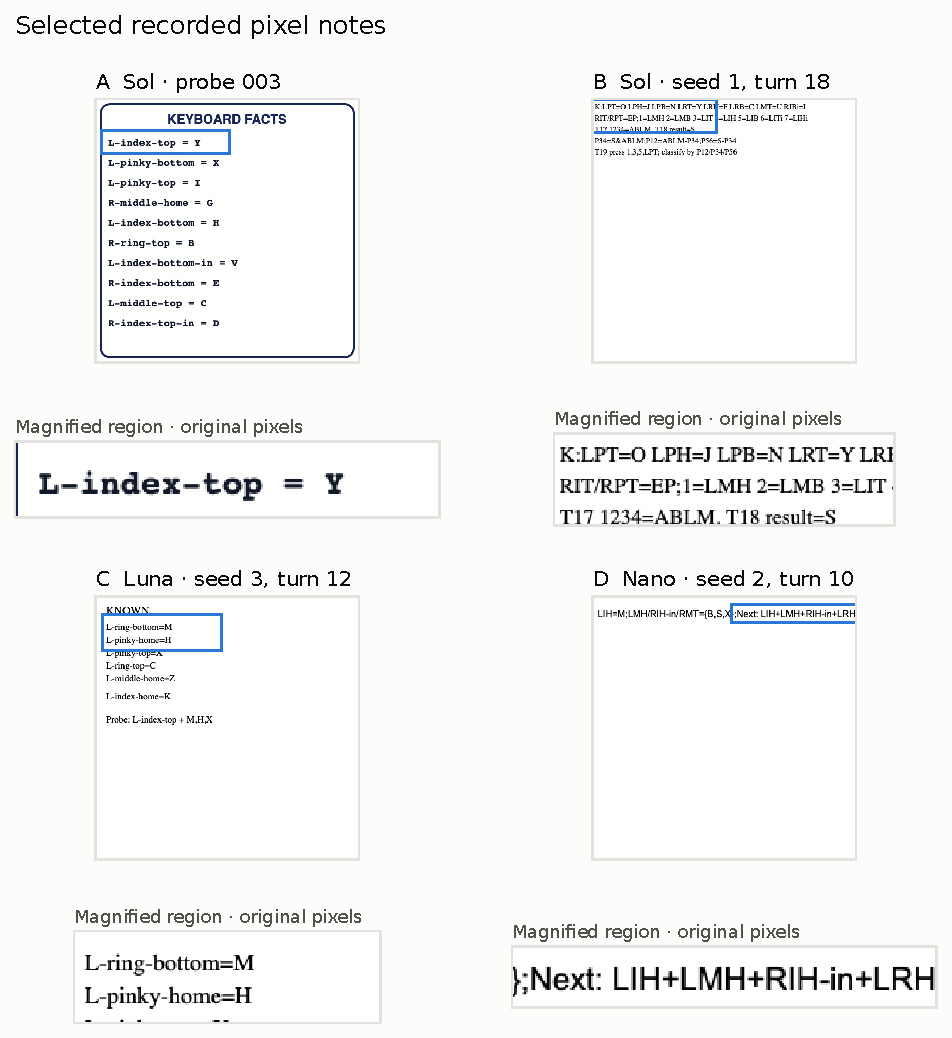
\includegraphics[width=\linewidth]{figures/relay_fig2_svg_notes.pdf}
\caption{Four selected stored pixel notes: a GPT-5.6 Sol transcription probe (A) and game notes from Sol (B), GPT-5.6 Luna (C) and GPT-5.4 Nano (D). Insets magnify the original pixels. Sol's titled, monospaced probe card was recovered without error; Luna's larger text leaves less room for content; Nano's single line clips at the canvas edge. These text-bearing examples do not establish whether spatial encoding strategies occur elsewhere in the corpus.}
\label{fig:svgnotes}
\end{figure}

Sol's perfect write--render--read recovery on the probe coexists with a lower game-score estimate. On the five shared seeds, SVG accuracy is $.608$ and $B{=}100$ text accuracy is $.923$, a paired difference of $-.32$ (\Cref{tab:svg}). The SVG cap of 2{,}500 bytes has no single equivalent text budget, so this is not a capacity-matched comparison. The game cell has $n{=}5$, and the SVG-minus-text contrast is unconfirmed (exact sign $p{=}.375$). Terra and the four added models were not tested in this channel.

The probe contains 10 independent facts, not mid-game set constraints. It differs from the game in both state complexity and query demand. Perfect recovery on this simpler probe does not explain the lower game point estimate or identify its cause. Both image and text interfaces require a replacement artifact on every turn. The selected images show self-authored text layouts; we did not classify spatial strategies across the corpus. These small-sample channel comparisons remain underpowered.

\subsection{Paired scaffold contrasts and pinned notation (exploratory)}\label{app:crossover}

Two different treatments have negative estimates at raw $p{=}.021$ (\Cref{tab:contrasts}): the schema for Luna ($-.22$ at $B{=}200$) and the form for Sol ($-.25$ at $B{=}100$). Neither survives family-wise correction. Sol's schema estimate is positive, as is Terra's (\Cref{tab:contrasts}). These results do not establish that imposed schemas harm stronger models as a class.

Luna's schema estimates are negative at every tested budget. One possible explanation is the need to translate between mnemonic addresses and key indices. A compact notation need not be easy for the model to use, and Luna's better-performing notes retain readable mnemonic addresses. The harness form also replaces Sol's existing strategy. These observations suggest possible mechanisms but do not identify one; at $n{=}10$, none of these contrasts survives correction. A follow-up is inexpensive: the three-condition screen at $B{=}100$ costs \$\relayfitcostnano--\$\relayfitcostsol{} per model at list prices. A confirmatory study would need a declared effect, power calculation and stopping rule.

\begin{figure}[!ht]
\centering
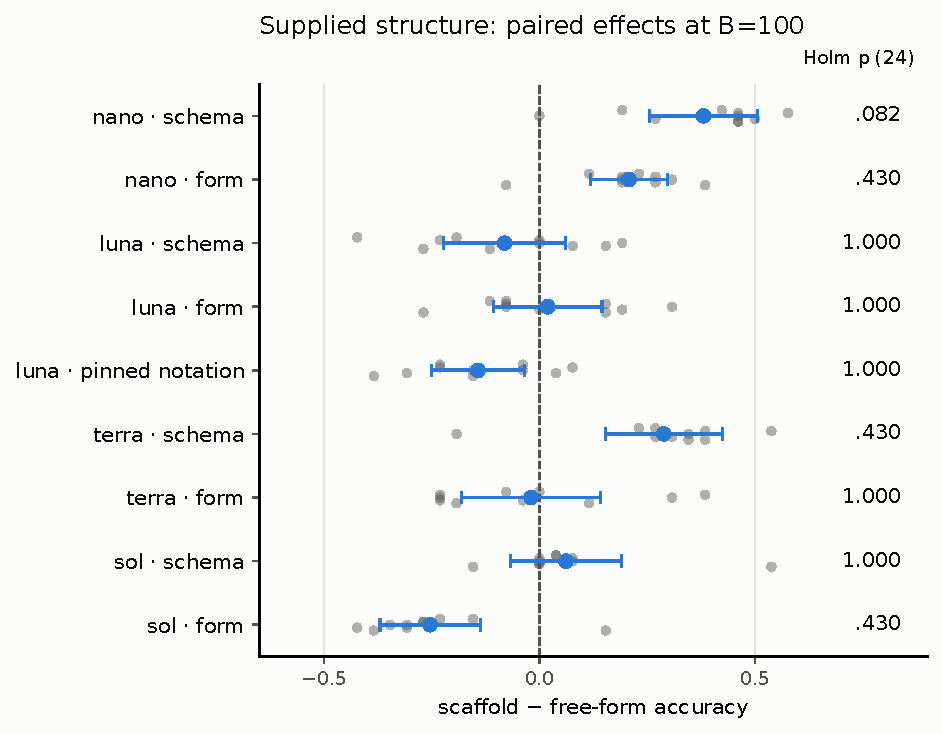
\includegraphics[width=\linewidth]{figures/relay_fig3_crossover.pdf}
\caption{Paired scaffold-minus-free-form differences in board accuracy (fraction of keys correct) at $B{=}100$, using seeds 0--9 ($n{=}10$). Points show mean and individual seed differences; intervals are 95\% $t$ intervals. Holm $p$ values use the full declared 24-test family. The pinned-notation row is for GPT-5.6 Luna only. These compare interface packages, not a cross-model interaction; no negative contrast survives family correction.}
\label{fig:crossover}
\end{figure}

\paragraph{Pinned-notation case study.}\label{app:lockin}
Designing a notation before play did not establish a benefit for the one model tested. Luna's pinned specification, the \emph{constitution} condition, has a lower mean than free-form notes at three of four budgets. Estimates range from $-.16$ to $+.01$; the smallest raw $p{=}.109$, and none survives correction. Luna designs specifications of 258--400 characters for note budgets of 50--200 (\Cref{app:constitution}), but the specification itself is outside the note budget. Its length therefore does not establish that the design is infeasible. A persistent but suboptimal convention is a possible explanation, not an identified mechanism. This is a single-model case study with unconfirmed differences.

\subsection{A constitution, verbatim (GPT-5.6 Luna; designed for \texorpdfstring{$B{=}100$}{B=100})}\label{app:constitution}
\begin{quote}\footnotesize\ttfamily\raggedright\sloppy
Keys are coded 0\textendash{}9,A\textendash{}P in the board-list order. Note format: `m=XXXXXXXXXXXXXXXXXXXXXXXXXX` (current key$\to$letter; `.` unknown); `h=abcd/EFGH` entries record each chord's 4 key codes and sorted result, newest first; append `!xyz` for rotated keys. Delete entries proven redundant. `q=abcd` is next planned chord; `l=` records locks. Use $\leq$100 chars.
\end{quote}
The \texttt{m=} layout field uses 28 characters and fits the 100-character note budget. The specification itself is free. It gives no separate bound for history entries and does not fully specify how to limit the auxiliary history and planning fields. The observed score comparisons do not establish a benefit from pinning the specification.

\FloatBarrier

\subsection{Interpretation and remaining experiments}\label{app:interpretation}
The declared tests do not resolve the frontier-model comparisons. A ranking requires enough informative paired instances to detect the intended differences, not necessarily a condition below the ceiling on every seed. For the frontier models, the 39-key board at $B{=}100$ remains an unrun candidate. The reference's full-state serialization peaked at 97 characters on its evaluated trajectories; that does not predict difficulty for frontier models.

Transmission chains motivate the note-format diagnostics \citep{kirby2001,kirby2008,acerbi2023,telephone2024,brokentelephone2025}. Fixed model weights do not rule out in-context adaptation, and we did not identify attractor dynamics or a cultural-evolution mechanism. A cross-model reader test and a representation that passes the fixed-codec negative control could test stronger claims about conventions.

Reference improvements must remain versioned. A fixed policy's attainable score can be exceeded. Adopting a model's encoding into a later codec does not revise that model's result against the earlier version. Both calibration generations are retained. Extending the protocol to another benchmark with a sound player remains a proposal.

\subsection{Extended related work}\label{app:related}

\paragraph{Agent memory: benchmarks and architectures}
Agent-memory benchmarks evaluate recall in a persistent agent's accumulating context or memory store: long conversations \citep{locomo2024}, multi-platform enterprise timelines \citep{memtrack2025}, dynamic environments \citep{gaia226,evoarena2026}, multi-session applications \citep{memoryarena2026,memgym2026}, and staleness detection \citep{stale2026}. Staleness detection shares \blindboard's premise that retrieving a fact does not establish whether it is still current. Relay resets the context on every turn and measures performance when the model must write the note that preserves its authored memory.

\citet{signals2026} vary memory architecture in a Lewis signaling game, a cooperative coordination task. They compare an overwritten 150-word scratchpad, fixed-capacity codebooks and a rolling 20-round history, and report that stateless agents' performance collapses at high channel capacity. This shows the importance of what is passed between calls, but the task requires neither hidden-state deduction nor budget certification and does not compare a ladder of scaffolds. Latent ``relay'' compression \citep{kvrelay2026} passes continuous key--value (KV) cache state between agents at specified compression ratios. The artifact is sub-symbolic, so there is no explicit notation to invent, inspect or track as it changes, as there is in Relay's human-legible channel.

A rate-distortion account of agent memory \citep{ratedistortion2026} provides a theory of decision-relevant compression. Our budget-matched reference supplies an attainable policy score, not an estimated rate-distortion frontier. Precision-aware memory benchmarking \citep{precisionmembench2026} separates retrieval correctness from answer correctness within a harness-maintained persistent belief store. Relay instead uses sound truncation of a full belief tracker to record attainable scores under a specified policy and free-input convention. Budget normalization can also change rankings: \citet{budgetrestoration2026} show that controlling the retrieval budget removes apparent advantages on full-text scientific memory. Relay fixes its budget in the protocol rather than normalizing scores afterward, and certifies the budgets at which a sound player succeeds.

\paragraph{Context compression and summarization memory}
Prompt-compression methods include token pruning \citep{llmlingua2023}, gist tokens \citep{gist2023}, recursive vector summarization \citep{autocompressors2023,icae2023}, and summarization trees \citep{raptor2024,wu2021books}. These methods compress supplied, static content once, for efficiency. Self-managed memory systems \citep{memgpt2023,generativeagents2023,latentctx2026} provide persistent stores with their own accounting rules. Budget limits also appear in \citet{retainconsolidate2026,memaudit2026,budgetbench2026}. \citet{retainconsolidate2026} choose, for each record, between retaining raw text and consolidating it as the store's budget tightens.

That choice assumes a persistent store. A relay instance instead writes one artifact from a single turn's context and never sees it again. The artifact is self-authored under a hard budget and passes through repeated author$\to$reader handoffs across complete context resets. We study the model's chosen encoding, its stability and its readability by fresh instances, rather than a compressor's retention rate.

\paragraph{Iterated learning, telephone games, and convention formation}
Iterated learning shows that transmission through a bottleneck can regularize languages \citep{kirby2001,kirby2008}, in neural agents as well as humans \citep{ren2020,chaabouni2020,lu2020seeded}. Large language models reproduce human content biases in transmission-chain retelling experiments \citep{acerbi2023}, the earliest such model study known to us. Model populations also form conventions \citep{conventions2024} and distort content across regeneration chains \citep{telephone2024,brokentelephone2025}; recursive training-loop analogues degrade as well \citep{shumailov2024}. \citet{colas2025} pass written advice across generations of learners in a complex task.

Relay studies replacement notes within one episode, with fixed model weights and checkable game state. Its surface-similarity metric does not independently validate conventions or establish that scarcity induces standardization. We make no universal priority claim for this combination.

\paragraph{Self-notes, handoffs, and self-authored artifacts}
Self-note and reflection methods let a persistent agent annotate its continuing context \citep{selfnotes2023,reflexion2023,expel2023,voyager2023,sleeptime2025}. Skill libraries preserve code rather than state \citep{voyager2023}. Chain-of-agents pipelines pass unbounded summaries for long-document tasks without budgets or certificates \citep{chainofagents2024}. Studies of self-authored structuring artifacts generally report benefits; model-authored specifications, for example, improve single-shot code generation \citep{selfspec2025}.

Relay's constitution condition offers a budgeted comparison, but only as an exploratory case. A specification designed once and repeated across turns produced lower means than free-form notes for the one model tested, without confirmed differences (\Cref{app:crossover}). \citet{constitutions2026} provide the closest comparison. They evaluate four constitutional regimes in a multi-agent survival game: adversarial, a human-written prosocial baseline (helpful/harmless/honest), model-designed, and evolutionarily refined. The model-designed constitution outperforms the human-written one ($S{=}.332$ versus $.249$) but scores below search refinement ($.556$).

These studies use different tasks and comparisons. Neither identifies a mechanism for Relay's unconfirmed Luna case study. Their constitutions govern behavior without a memory constraint; Relay's constitution specifies notation for notes that must fit a hard budget. Its causal effect remains unresolved.

\paragraph{Text through pixels}
SVG generation and understanding have dedicated benchmarks \citep{svgenius2025}. Vision-language models (VLMs) perform worse when reading rendered text than native text \citep{vistabench2026,readingnotthinking2026}. Other work deliberately renders text as pixels for context compression \citep{glyph2025,deepseekocr2025} or visual reasoning scratchpads \citep{renderofthought2026,opticalreasoning2026}. These studies use their own reading and session protocols. Latent visual channels between agents require trained or white-box access \citep{visionwormhole2026,hylat2026}.

In Relay's pixel channel, the image is the only carried model-authored note between independent instances with fixed weights, and the writer chooses its encoding. A separate transcription probe measures the combined write$\to$render$\to$read fidelity. We report recovery on that simpler probe alongside exploratory game outcomes, without identifying a causal modality effect.

\subsection{Frontier models at tight budgets}\label{app:frontier}
\begin{table}[htbp]
\centering
\small
\caption{Mean board accuracy (fraction of keys correct) for the three frontier added models, their retained-reasoning controls and the budget-matched sound reference. Initial free-form and reference means use seeds 0--9; the 40-seed reference mean at $B{=}30$ is $\relayfloorbthirty$. F14 gives free-form-minus-retained differences; the lower panel gives paired model differences. F15 uses seeds 0--9; F16 uses fresh seeds 10--29 at $B{=}50$; F17 uses the 60-turn-cap condition at $B{=}100$. Each family is Holm-corrected within itself. Turn counts in the headings are caps; early guesses are allowed. The reference was not run with the 60-turn cap.}
\label{tab:frontier}
% Generated by scripts/relay_analysis.py. Do not hand-edit.
\begin{tabular}{@{}lrrrrrrrr@{}}
\toprule
 & \multicolumn{3}{c}{free-form, 20 turns} & 60 turns & & \multicolumn{2}{c}{F14: $\Delta$ (Holm $p$)} \\
\cmidrule(lr){2-4}\cmidrule(lr){5-5}\cmidrule(l){7-8}
model & $B{=}100$ & $B{=}50$ & $B{=}30$ & $B{=}100$ & retained & $B{=}50$ & $B{=}30$ \\
\midrule
\solicon\ GPT-6 Sol & .969 & .935 & .538 & .973 & 1.000 & $-.065$ (.250) & $-.462$ (.012) \\
Gemini 3.8 Flash & .992 & .765 & .431 & .992 & 1.000 & $-.235$ (.188) & $-.569$ (.020) \\
Opus 5.5 & .992 & .946 & .500 & .992 & 1.000 & $-.054$ (.250) & $-.500$ (.020) \\
\midrule
sound reference & 1.000 & 1.000 & .519 & -- & & & \\
\bottomrule
\end{tabular}
\par\medskip
\begin{tabular}{@{}lrrrr@{}}
\toprule
 & \multicolumn{2}{c}{F15: seeds 0--9} & F16: seeds 10--29 & F17: 60 turns \\
\cmidrule(lr){2-3}\cmidrule(lr){4-4}\cmidrule(l){5-5}
pair: $\Delta$ (Holm $p$), paired by seed & $B{=}50$ & $B{=}30$ & $B{=}50$ & $B{=}100$ \\
\midrule
Gemini 3.8 Flash $-$ \solicon\ GPT-6 Sol & $-.169$ (1.000) & $-.108$ (1.000) & $+.004$ (1.000) & $+.019$ (1.000) \\
Opus 5.5 $-$ \solicon\ GPT-6 Sol & $+.012$ (1.000) & $-.038$ (1.000) & $+.127$ (.680) & $+.019$ (1.000) \\
Opus 5.5 $-$ Gemini 3.8 Flash & $+.181$ (1.000) & $+.069$ (1.000) & $+.123$ (.680) & $+.000$ (1.000) \\
\bottomrule
\end{tabular}

\end{table}

\textbf{Tighter budgets lower frontier scores without establishing a ranking.} The three frontier models ran free-form notes at $B{=}50$ and $B{=}30$ on the same seeds under F14 and F15, both declared before collection. F16 added twenty fresh seeds at $B{=}50$, and F17 used $B{=}100$ with a 60-turn cap; both were declared before their own collection (\Cref{tab:frontier} and \Cref{fig:frontier}). F14 compares free-form notes with retained reasoning across six tests (three models, two budgets). F15 contains six pairwise model comparisons on seeds 0--9. F16 repeats the $B{=}50$ pairwise comparisons on seeds 10--29, and F17 compares the models with the 60-turn cap; each contains three tests.

At $B{=}50$ on the initial seeds, GPT-6 Sol scores $\relayaddfreefiftysolsix$, Opus 5.5 $\relayaddfreefiftyopus$ and Gemini 3.8 Flash $\relayaddfreefiftyflash$. No model's loss relative to its retained control is significant after correction (F14; smallest Holm $p\relayfourteenfiftyminholm$). At $B{=}30$, each loses about half its retained-control score. The F14 differences are $\relayfamfourteensolsixthirtydelta$ for GPT-6 Sol, $\relayfamfourteenflashthirtydelta$ for Gemini 3.8 Flash and $\relayfamfourteenopusthirtydelta$ for Opus 5.5; each Holm $p{\leq}\relayfourteenthirtymaxholm$.

Their $B{=}30$ means are $\relayaddfreethirtysolsix$, $\relayaddfreethirtyflash$ and $\relayaddfreethirtyopus$, respectively, compared with the reference's $\relayfloorbthirtyshared$ on the same ten seeds. GPT-6 Sol is slightly above that reference mean; GPT-5.6 Sol also scored nearby ($\relaysolbthirty$). This proximity is descriptive, not evidence of equality. No pairwise model difference survives correction at either budget (F15; largest difference $\relayfifteenmaxabs$, Holm $p\relayfifteenminholm$). Per-seed scores at $B{=}30$ range from $\relaythirtyseedmin$ to $\relaythirtyseedmax$; these ten seeds do not establish a ranking.

Twenty fresh seeds at $B{=}50$ do not establish a ranking either (F16, declared before their collection). Gemini 3.8 Flash's initial deficit does not recur: it scores $+\relayfamsixteenflashsolsixdelta$ relative to GPT-6 Sol. Opus 5.5 leads both by about an eighth: $+\relayfamsixteenopussolsixdelta$ against GPT-6 Sol and $+\relayfamsixteenopusflashdelta$ against Gemini 3.8 Flash. The $t$ intervals, $[\relayfamsixteenopussolsixlo, \relayfamsixteenopussolsixhi]$ and $[\relayfamsixteenopusflashlo, \relayfamsixteenopusflashhi]$, only just exclude zero, but the primary sign test does not confirm either contrast. Against GPT-6 Sol, Opus 5.5 wins \relayfamsixteenopussolsixpos{} seeds, loses \relayfamsixteenopussolsixneg{} and ties \relayfamsixteenopussolsixties{} near the ceiling (Holm $p\relayfamsixteenopussolsixholm$). Over all \relayaddfreefiftyallnopus{} seeds at $B{=}50$, Opus 5.5 averages $\relayaddfreefiftyallopus$, GPT-6 Sol $\relayaddfreefiftyallsolsix$ and Gemini 3.8 Flash $\relayaddfreefiftyallflash$.

The 60-turn-cap condition also leaves the ranking unresolved (F17, declared before collection). At $B{=}100$, GPT-6 Sol scores $\relayaddfreelongsolsix$, Gemini 3.8 Flash $\relayaddfreelongflash$ and Opus 5.5 $\relayaddfreelongopus$. These means are near their standard-condition estimates, but equivalence was not tested. Every pair ties on most seeds (all Holm $p\relayfamseventeenopussolsixholm$). The models did not complete 60 turns: GPT-6 Sol guessed on turns $\relaylongsolsixguessmin$--$\relaylongsolsixguessmax$, Gemini 3.8 Flash on $\relaylongflashguessmin$--$\relaylongflashguessmax$, and Opus 5.5 on $\relaylongopusguessmin$--$\relaylongopusguessmax$. This condition tests a larger available horizon with voluntary stopping, not sustained performance through 60 handoffs.
